\documentclass[11pt,a4paper]{article}
\usepackage[T1]{fontenc}
\usepackage[utf8]{inputenc}
\usepackage[margin=24mm]{geometry}
\usepackage{amsmath,amssymb,mathtools,booktabs,array,graphicx,xurl}
\usepackage[colorlinks=true,linkcolor=blue,urlcolor=blue,citecolor=blue]{hyperref}
\usepackage{enumitem}
\setlist{itemsep=3pt,topsep=4pt}
\setlength{\parindent}{0pt}
\setlength{\parskip}{6pt}
\setlength{\emergencystretch}{3em}
\setcounter{tocdepth}{1}
\newcommand{\pos}[1]{\left[#1\right]_+}
\newcommand{\E}{\mathbb E}
\DeclareMathOperator{\clip}{clip}
\hypersetup{pdftitle={From farm and weather data to solar and battery trading decisions},pdfauthor={PV--BESS research programme}}
\title{From Farm and Weather Data\\to Solar and Battery Trading Decisions}
\author{Data, forecast paths and auction participation}
\date{4 November 2026}
\begin{document}
\maketitle
\begin{abstract}
A solar producer must commit electricity before its production is known.
Battery storage provides flexibility, while successive auctions create
opportunities to revise the contracted position as weather information
improves. We study this problem using four northern-Italian farms, historical
production and irradiance, regularly updated weather forecasts, and 50-member
weather ensembles. Weather is converted into possible AC production paths;
these paths support physically feasible trading and battery decisions.
Participation studies compare every nonempty subset of the day-ahead and three
intraday auctions, with each strategy carrying its own state through time.
This document explains the available data, the forecast-to-decision process,
and the first participation results. The full optimization and supporting
equations are collected in appendices.
\end{abstract}
\tableofcontents
\newpage

\section{The problem and our core idea}
A photovoltaic farm and a battery share a grid connection. Solar generation
can be exported, stored or curtailed; the battery can also charge from grid
imports. The producer sells and buys energy in the Italian day-ahead auction
(DA) and three intraday auctions (IDA1, IDA2 and IDA3). An order becomes binding
when submitted. Later auctions can adjust the resulting position, while
battery operation helps deliver it under uncertain solar production.

Our core idea is to connect the information available at each auction with
\emph{the decisions that can still be changed}. We transform eligible weather
forecasts into production paths, optimize the remaining market opportunities
and battery operation together, submit the current order, and repeat as new
information arrives. Earlier commitments remain fixed. The actual battery
state links the decisions across delivery intervals and days.

The model maximizes expected remaining auction revenue less battery wear and
trading costs, subject to energy conservation, exclusive charging/discharging,
stored-energy bounds and the shared grid limit. The full optimization is in
Appendix~\ref{app:auction}.

This allows us to ask three concrete questions. How does participation in
additional auctions change the achievable operating outcome? What changes when
a single production forecast is replaced by an ensemble? How much does joint
planning of remaining auctions contribute relative to optimizing one auction
at a time? We assess profit together with imbalance, curtailment, wear and
ending stored energy.

\section{The available data}
\subsection{Four farms and their historical records}
The dataset covers four anonymous farms in the northern-Italian bidding zone.
Installed power is measured on the AC side. The supplied metadata describe
fixed arrays and single-axis trackers:
\begin{center}\small
\begin{tabular}{rllrr}
\toprule Farm & AC capacity (MW) & Declared technology & Battery (MWh) & Power (MW)\\\midrule
1   & 0.95328 & Fixed array & 0.75 & 0.5\\
345 & 1.52460 & Fixed array & 1.00 & 0.5\\
901 & 4.16000 & Bifacial single-axis tracker & 2.00 & 1.0\\
910 & 6.63800 & Single-axis tracker & 5.00 & 2.5\\
\bottomrule\end{tabular}\end{center}
The batteries are hypothetical study assets. Their energy and power ratings,
7--93\% state-of-charge range, 90\% round-trip efficiency and connection limits
are modeling assumptions. The farm metadata also provide nominal orientation,
tilt and elevation. Exact farm coordinates are unavailable, so solar-position
calculations use documented geographical proxies; fitted effective geometry or
rear-irradiance assumptions can differ from the metadata label.

Historical records run from 1 January 2025 to 31 August 2026 on a 15-minute
UTC grid: 58,368 timestamps for each farm. They contain AC power, historical
satellite global horizontal irradiance (GHI), and historical diffuse fraction.
This is the time grid's size, rather than a count of independently verified,
complete measurements. Power is converted once from kW to MW; multiplying by
the interval duration gives energy in MWh.

Production quality and availability matter to both forecasting and trading.
Reviewed modeling views distinguish retained measurements, approved synthetic
replacements, seasonal night zeros and excluded intervals. Historical-GHI
reconstructions provide explicitly identified counterfactual production where
used. Raw historical data, reviewed targets and reconstructed production have
different evidential meanings. Forecast training and replay therefore retain
their target policy and provenance.

\subsection{Updated deterministic weather forecasts}
The main weather archive contains 2,440 initialization times, every six hours,
from 30 December 2024 to 31 August 2026. Each initialization supplies 49 hourly
lead coordinates, from zero to 48 hours, for every farm. The weather fields
include global and direct horizontal radiation, total and layered cloud cover,
air temperature, dew point, wind components at 10 and 100 metres,
precipitation, snow-water equivalent and visibility.

A forecast is identified by its initialization and lead time; their sum gives
the valid time. Several issues can predict the same delivery interval. This
provides a record of forecast revision as delivery approaches. The four daily
issues are successive information updates, each supplying one deterministic
weather trajectory.

Hourly radiation represents an interval mean, and precipitation an hourly
accumulation. Alignment with the quarter-hour delivery grid respects those
semantics. Issue time, assumed publication time and delivery time are retained
separately. In the studies, forecasts become available six hours after
initialization; this is an explicit release assumption.

\subsection{Weather ensembles}
Two separate archives supply \emph{50 weather members for the same issue and
lead times}, with the same four farms and 0--48-hour lead coordinates:
\begin{center}\small
\begin{tabular}{lll}
\toprule Archive & Available 00 UTC initializations & Members / hourly leads\\\midrule
Winter & 31 Dec. 2025--31 Jan. 2026 (32 issues) & 50 / 49\\
Late summer & 1 Aug.--30 Sept. 2026 (61 issues) & 50 / 49\\
\bottomrule\end{tabular}\end{center}
These members represent alternative weather trajectories within one forecast
issue. Keeping a member's identity through the horizon retains its supplied
temporal evolution, including the duration of cloudy and sunny periods. The
spread supplies uncertainty information that a single deterministic forecast
cannot describe. Equal scenario weights are a modeling choice; coverage and
calibration require separate assessment.

The participation studies freeze the ensemble initialized at 00 UTC on the
\emph{preceding delivery day}. The winter archive includes 31 December, which
supports 1 January delivery. The late-summer archive begins on 1 August and
therefore supports this convention from 2 August. Its September weather issues
extend beyond the available farm-production record used here.

\subsection{Market observations}
Historical clearing curves cover DA and the three intraday auctions, with
imbalance-settlement prices used to value actual delivery deviations. Native
product durations and daylight-saving changes are preserved. Physical operation
uses quarter-hours; earlier hourly DA products remain single traded products
when mapped onto that finer grid.

The participation comparisons use actual future auction prices as a common
price-information benchmark. This isolates choices about market access,
production forecasts and physical flexibility under that benchmark. Their
profits must be interpreted with this price-foresight assumption. Developing
price forecasts is a further route toward operational decisions.

\section{From weather information to production and decision paths}
\subsection{Selecting information at the auction cutoff}
The study uses the following market timeline, in Italian local time. Decisions
are taken five minutes before each gate:
\begin{center}\small
\begin{tabular}{llll}
\toprule Auction & Gate & Delivery covered & Latest typical weather issue\\\midrule
DA & Previous day, 12:00 & Whole next day & Previous day, 00 UTC\\
IDA1 & Previous day, 15:00 & Whole next day & Previous day, 06 UTC\\
IDA2 & Previous day, 22:00 & Whole next day & Previous day, 12 UTC\\
IDA3 & Delivery day, 10:00 & Noon to midnight & Delivery day, 00 UTC\\
\bottomrule\end{tabular}\end{center}
The last column follows the six-hour release assumption and requires sufficient
remaining-horizon coverage. At every cutoff, the deterministic forecast is
updated to the latest eligible issue. The 50 ensemble paths retain the frozen
preceding-day issue, so their information age differs from the updating
forecast. This distinction is part of the comparison design.

\subsection{Converting weather into AC generation}
The physical forecast first derives direct and diffuse irradiance components,
then projects them onto the array or tracker plane. It estimates module
temperature from air temperature, wind and plane-of-array irradiance, computes
DC production and converts it to AC power. Output is bounded by the farm AC
rating and forced to zero during the specified seasonal nighttime windows.
Effective conversion parameters can be estimated from historical data.

Statistical and neural models provide another mapping from weather, calendar,
lead-time and farm information to AC production. Historical power and irradiance
support fitting and diagnosis; evaluation uses the forecast weather available
for the delivery interval. Where learning uses historical irradiance, the shift
to forecast irradiance is stated explicitly. Chronological training, selection
and evaluation periods are kept distinct. Measured-only and reconstructed-target
scores answer different questions.

Each ensemble weather member passes separately through the selected conversion
model, producing a complete AC power path on the delivery grid. The study's
51-path input combines these 50 paths with the updating deterministic forecast.
This ensemble construction differs from generating paths by independently
sampling marginal quantiles at each time. The full path matters to a battery:
a sustained production shortfall can exhaust stored energy even when its
pointwise forecast spread resembles that of a shorter shortfall.

\begin{figure}[htbp]
\centering
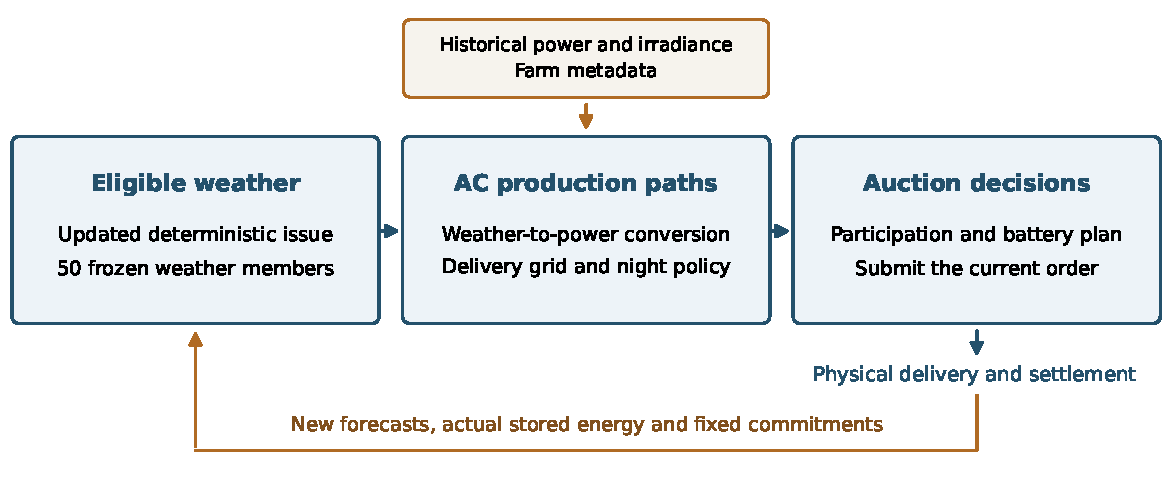
\includegraphics[width=\textwidth]{docs/figures/research_report/data_to_decisions.pdf}
\caption{Historical records support the production mapping and evaluation.
Eligible weather issues supply forecast paths; those paths support auction
and physical decisions. Realized delivery supplies the carried battery state.}
\end{figure}

\subsection{Turning forecast paths into a trading policy}
At a given cutoff, a production path is a possible external input. A decision
path consists of auction quantities and feasible battery/solar actions along
the represented information history. Scenarios with the same information must
share the decisions made before they can be distinguished. Future production
is therefore not disclosed merely by representing several paths.

In the strict ensemble participation studies, orders and planned battery
commands are common across all 51 production paths; curtailment can adapt to
available production. Every represented path must support the contracted
delivery. With identical price paths and the stated curtailment recourse, useful
solar injection is bounded by the pointwise minimum across production paths.
This makes the strict formulation conservative. An ensemble of forecasts does
not automatically imply adaptive future battery decisions.

Integrated planning optimizes the remaining participating auctions together.
Only the closing auction's quantity is submitted. At the next gate, that order
is fixed and provisional later orders are reoptimized with new eligible
forecasts. During delivery, commitment tracking adjusts physical battery power
within its energy, power and grid limits. Actual SOC, submitted commitments,
wear and transaction-fee state carry into subsequent decisions and days. A
forecast projection supplies the starting state for tomorrow's plan while
today's delivery is still in progress; the realized state governs execution.

\section{The auction participation studies}
\subsection{What is compared}
Four optional auctions give $2^4-1=15$ nonempty participation profiles: four
single-auction profiles, six pairs, four triples and the all-auction profile.
An auction omitted from a profile supplies no submission opportunity. The
remaining gates retain their chronological order and delivery eligibility.

Every profile has its own continuous physical and financial trajectory. At the
start of the study the initial state is common within a farm; afterward each
strategy's actions determine its own SOC and later feasible trades. The
January 2026 comparison starts at 90\% SOC and carries state over 31 days.
Planning uses a 50\% terminal target and a 40\% floor; forecast error and physical
execution can yield different realized ending inventories.

The study runs each profile with an updating deterministic production forecast
and with the 51-path input. Two references clarify the mechanism:
\begin{itemize}
\item \textbf{Sequential all-auction planning:} participate in every auction,
but optimize only the current auction's quantities at each gate. Later gates
can still revise the physical plan and add their own trades.
\item \textbf{Perfect-production reference:} disclose future production while
retaining the same asset and actual-price benchmark. It shows the outcome of
that information counterfactual under its specified planning convention.
\end{itemize}
Integrated and sequential planning thus differ even when they have the same
auction access. With price foresight, the integrated model can anticipate
cross-auction spreads and coordinate earlier purchases/sales with later ones.
The resulting difference combines that economic opportunity with forecast and
physical effects.

\subsection{First results and their interpretation}
An earlier January 2025 farm-910 study compared all 15 profiles on independently
initialized days. Its all-auction integrated profile ranked first, with mean
profit EUR 3,520.06/day and total EUR 109,121.72 over 31 days. The continuous
January 2026 studies then retained the actual trajectory across days for all
four farms and both forecast variants. These two designs have different state
assumptions and are evaluated separately.

The following January 2026 cash totals summarize three key participation
choices. D denotes deterministic production and E the strict 51-path input.
All columns use the same actual-price benchmark:
\begin{center}\small
\begin{tabular}{rrrrr}
\toprule Farm & DA only D & Sequential all D & Integrated all D & Integrated all E\\
 & EUR & EUR & EUR & EUR\\\midrule
1 & 1,648.99 & 1,848.22 & 10,216.33 & 10,197.54\\
345 & 6,494.09 & 6,916.97 & 20,306.16 & 18,555.04\\
901 & 16,467.77 & 16,904.75 & 53,708.73 & 49,397.35\\
910 & 19,804.62 & 20,500.95 & 78,971.91 & 76,171.83\\
\bottomrule\end{tabular}\end{center}
The large integrated/sequential difference is consistent with the ability to
plan actual-price spreads across auctions. It cannot be attributed solely to
more accurate solar forecasts. Figure~\ref{fig:participation} shows the full
profile comparison for farm 1; it also makes the contribution of particular
auction combinations visible.

\begin{figure}[htbp]
\centering
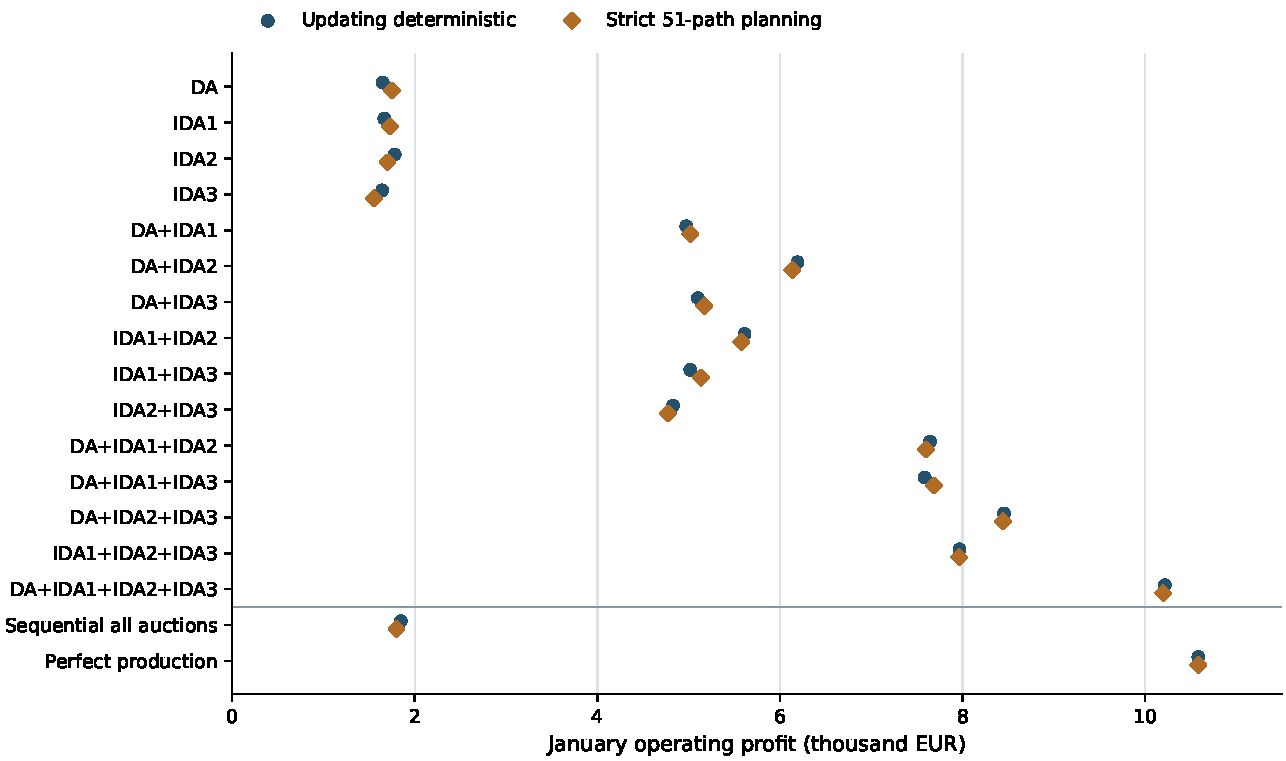
\includegraphics[width=0.96\textwidth]{docs/figures/research_report/participation_profiles.pdf}
\caption{Farm 1, continuous January 2026: monthly operating profit for all
15 auction subsets and the two references. Dots show the deterministic and
strict 51-path inputs. Earlier orders remain fixed and each profile carries
its own battery state. Perfect production is a separately labelled hindsight
reference.}\label{fig:participation}
\end{figure}

Strict ensemble planning reduces absolute imbalance for the all-auction
profile on all four farms. For farm 1 it changes 5.818 to 1.577 MWh, with wear
EUR 520.52 versus EUR 525.84 and final SOC 33.50\% versus 43.49\%. For farms
345, 901 and 910, absolute imbalance changes from 2.447 to 0.780, 23.099 to
4.320, and 70.412 to 21.643 MWh respectively. Cash profit decreases in each
all-auction comparison. This illustrates how uncertainty representation changes
market exposure and use of physical flexibility; reducing imbalance alone does
not determine the economically preferred profile.

Separate full January and August production-input comparisons provide winter
and summer cases; August starts on the second because the required preceding
ensemble issue is absent for its first day. Each month starts independently.
Reported outcomes include daily profit distributions, settlement cash,
curtailment, charge/discharge, wear and ending SOC. Cash profit excludes capital
cost and terminal inventory valuation. The rankings are retrospective and use
actual-price foresight; historical model selection and the target provenance
further limit an operational interpretation.

\section{What this framework enables next}
The available data connect forecast revision, production uncertainty and
sequential participation within one physical chronology. The next questions
are how forecast calibration and price prediction change those participation
results, and how receding-horizon battery control uses new observations between
auction gates. These developments build on the same data-to-path-to-decision
structure. Longer comparisons must retain common dates, target provenance,
information timing and ending-inventory accounting.

\clearpage
\appendix

\section{Full residual auction optimization}
\label{app:auction}
\subsection{Sets, parameters and signs}
Let $t\in\mathcal T$ index the remaining physical intervals of a delivery day,
$\Delta_t$ their duration in hours, $s\in\mathcal S$ scenarios with probabilities
$w_s$, and $a\in\mathcal A_k$ auctions still open at decision $k$.
$\mathcal T_a$ is auction $a$'s eligible delivery set. Native products group
physical intervals; their identifiers retain daylight-saving offsets.

Solar availability is $V_{s,t}$ MW AC, battery capacity $E$ MWh, power limit
$\bar P$ MW, energy bounds $E^{\min},E^{\max}$, efficiencies $\eta_c,\eta_d$
and hourly self-discharge $\sigma$. The grid limits are $P^{\rm imp},P^{\rm exp}$.
$Q_t^{\rm fix}$ is the signed MWh position from all earlier submitted quantities,
including still-unpriced orders. Positive trade/grid signs mean sale/export.
Auction price coefficients are $\pi_{a,s,t}$ in EUR/MWh.

Controls $c_{n,t},d_{n,t}$ are charging/discharging MW; $z_{n,t}$ is a charging
binary. Curtailment is $u_{m,t}$ MW, injection $i_{s,t}$ MW, grid exchange
$g_{s,t}$ MW and internal energy $e_{s,t}$ MWh. $q_{a,n,t}$ is a signed auction
adjustment in MWh. Node maps $n_t(s),n_a(s),m_t(s)$ encode observable history.
Leaf values below refer to their node-owned variables, so indistinguishable
histories cannot take different actions.

\subsection{Complete base problem}
For throughput wear $D_s=c_{\rm thr}\sum_t(c_{s,t}+d_{s,t})\Delta_t$ and
optional import cost $I_s=f\sum_t\pos{-g_{s,t}}\Delta_t$, the residual model is
\begingroup\small
\begin{align}
 \max\quad &\sum_sw_s\left[
    \sum_{a\in\mathcal A_k}\sum_{t\in\mathcal T_a}\pi_{a,s,t}q_{a,n_a(s),t}
       -D_s-I_s-C_s^{\rm trade}\right] \label{eq:short-objective}\\
 \text{s.t.}\quad
 &i_{s,t}+u_{m_t(s),t}=V_{s,t},\quad i_{s,t}\ge0,\quad u_{m_t(s),t}\ge0,
                                                         &&\forall s,t,\\
 &g_{s,t}=i_{s,t}+d_{n_t(s),t}-c_{n_t(s),t},
                                                         &&\forall s,t,\\
 &-P^{\rm imp}\le g_{s,t}\le P^{\rm exp},                  &&\forall s,t,\\
 &0\le c_{n,t}\le\bar Pz_{n,t},\quad
   0\le d_{n,t}\le\bar P(1-z_{n,t}),\quad z_{n,t}\in\{0,1\},&&\forall n,t,\\
 &e_{s,t+1}=(1-\sigma)^{\Delta_t}e_{s,t}
       +\eta_cc_{n_t(s),t}\Delta_t-d_{n_t(s),t}\Delta_t/\eta_d,
                                                         &&\forall s,t,\\
 &E^{\min}\le e_{s,t}\le E^{\max},\quad e_{s,0}=e^k,       &&\forall s,t,\\
 &Q_{s,t}=Q_t^{\rm fix}+\sum_{a:t\in\mathcal T_a}q_{a,n_a(s),t},
                                                         &&\forall s,t,\\
 &g_{s,t}\Delta_t=Q_{s,t},                                &&\forall s,t,\\
 &-P^{\rm imp}\Delta_t\le q_{a,n,t}\le P^{\rm exp}\Delta_t,&&\forall a,n,t\in\mathcal T_a,\\
 &-P^{\rm imp}\Delta_t\le Q_t^{\rm fix}
           +\sum_{b\le a:t\in\mathcal T_b}q_{b,n_b(s),t}
            \le P^{\rm exp}\Delta_t,                     &&\forall a,s,t,\\
 &q_{a,n,t}/\Delta_t=q_{a,n,t'}/\Delta_{t'},
                  &&t,t'\text{ in the same native product}.\label{eq:short-product}
\end{align}
\endgroup
Only eligible quantities exist. The last equality ties average power within a
native product; on equal quarter-hours it ties MWh shares directly. Fixed
initial energy can be observed or a forecast projection to the eligible
boundary. A configured terminal equality $e_{s,T}=e_F$ and/or floor
$e_{s,T}\ge e_{\rm floor}$ is added where the study requires it. A planning
terminal target does not itself force an algebraic feedback controller to end
at that realized energy.

For progressive transaction tariff $F_m$, previously submitted monthly gross
volume $V_m$ and new gross volume $G_{m,s}=\sum_{a:m(a)=m,t}|q_{a,n_a(s),t}|$,
\begin{equation}
 C_s^{\rm trade}=\sum_m\{F_m(V_m+G_{m,s})-F_m(V_m)\}.
\end{equation}
Exact absolute-value and piecewise-linear graphs are required if reachable
marginal tariff bands are decreasing; a convex epigraph alone is insufficient.
The month is the submission month, not necessarily the delivery month.
Earlier auction cash and incurred wear are sunk and absent from
\eqref{eq:short-objective}. Only the closing auction's order is submitted;
other quantities are revisable plans. Sequential planning replaces
$\mathcal A_k$ by the single current auction.

\subsection{Exact envelope for the strict ensemble problem}
Under exact delivery, common trades/battery controls, identical price paths and
compatible instantaneous curtailment recourse, $i_t$ is shared and
\begin{equation}
 0\le i_t\le\min_sV_{s,t},\qquad u_{s,t}=V_{s,t}-i_t.
\end{equation}
This gives an exact reduced feasible set and objective. It does not apply to
general adaptive or imbalance-enabled problems, and discarding low-probability
paths is not part of the equivalence.


\section{Battery wear, control and realized accounting}
\subsection{Wear models}
For replacement value $R$, reference internal cycle depth $d_0$, life $N$ and
capacity $E$, AC throughput wear can be calibrated as
\begin{equation}
 c_{\rm thr}=\frac{R}{Nd_0E(1/\eta_c+\eta_d)},\qquad
 D=c_{\rm thr}\sum_t(c_t+d_t)\Delta_t.
\end{equation}
An optional segmented depth model uses stress $\Phi(d)=\alpha d^\beta$,
$\beta\ge1$, $J$ segments and marginal discharge cost
\begin{equation}
 m_j=\frac{RJ}{\eta_dE}\{\Phi(j/J)-\Phi((j-1)/J)\},
 \qquad D=\sum_{t,j}m_jd_{j,t}\Delta_t.
\end{equation}
Segment energy transitions sum to aggregate energy; shallow-first charging and
discharging priorities preserve cycle-depth memory. The segment vector carries
between decisions and cannot generally be recovered from SOC alone. This is
an approximation to cycle wear, not dynamic capacity fade or thermal/calendar
aging~\cite{xu}.

\subsection{Feedback, chronology and profit}
Commitment tracking uses target $g_t^*=Q_t^{\rm sub}/\Delta_t$ and interval PV.
Feasible charge and discharge are bounded by
\begin{equation}
 C_t=\min\!\left(\bar P,\frac{\pos{E^{\max}-\rho_te_t}}{\eta_c\Delta_t}\right),
 \quad D_t=\min\!\left(\bar P,\frac{\eta_d\pos{\rho_te_t-E^{\min}}}{\Delta_t}\right).
\end{equation}
It adjusts net battery power toward the grid target, recovers curtailed PV
where headroom permits, and enforces connection limits. Interval-average PV feedback is an idealized information assumption.
Executed battery state, curtailment and deviations are retained at every interval.

Realized accounting uses
\begin{align}
 \delta_t&=g_t^{\rm real}\Delta_t-Q_t^{\rm sub},\\
 J^{\rm real}&=\sum_{a,t}\pi^{\rm real}_{a,t}q^{\rm sub}_{a,t}
 +\sum_t\bigl(\lambda_t^+\pos{\delta_t}-\lambda_t^-\pos{-\delta_t}\bigr)
 -D^{\rm real}-I^{\rm real}-C^{\rm trade,real}.
\end{align}
With a single settlement price this reduces to $\lambda_t\delta_t$.
Forecast penalties, tail-risk terms and terminal continuation values are absent
from realized cash. Final energy is reported separately. The state and binding
positions carry across days; no daily physical reset occurs in a continuous
comparison.


\section{Forecast construction and information timing}
\subsection{Issue, availability and delivery}
For forecast initialization $\tau_v$, lead $h$ and availability $A_v$, define
\begin{align}
 t_{v,h}&=\tau_v+h,\qquad A_v=\tau_v+6\text{ hours},\\
 v^*(k)&=\max\{v:A_v\le k,\ \text{required delivery horizon covered}\}.
\end{align}
The deterministic production forecast at cutoff $k$ is
$V_{0,t}^{(k)}=f_{\theta}(X_{v^*(k),t},M)$, where $M$ denotes farm assumptions.
For delivery day $d$, let $v_d$ be the preceding day's 00 UTC ensemble issue.
The path input is
\begin{equation}
 V_{s,t}^{(k)}=f_\theta(X_{v_d,s,t},M),\quad s=1,\ldots,50,
 \qquad w_s=\frac1{51},\quad s=0,\ldots,50.
\end{equation}
The deterministic path updates while the weather-ensemble issue is fixed for
the day. Model availability and observation delays are additional eligibility
conditions; retrospective fitted models retain their historical-use label.

\subsection{Physical and statistical production mappings}
For GHI, horizontal beam irradiance BHI and solar zenith $\theta_z$, the
physical conversion uses the symbolic relationships
\begin{align}
 G_{\rm DHI}&=G_{\rm GHI}-G_{\rm BHI},\qquad
 G_{\rm DNI}\simeq G_{\rm BHI}/\cos\theta_z,\\
 G_{\rm POA}&=G_{\rm beam}+G_{\rm sky}+G_{\rm ground},\\
 T_{\rm mod}&=T_{\rm air}+G_{\rm POA}/(U_0+U_1v),\\
 P_{\rm DC}&=\max\!\left(0,\frac{P_{\rm AC,rated}}{\eta_{\rm ref}}
   \frac{G_{\rm POA}}{1000}[1+\gamma(T_{\rm mod}-T_{\rm ref})]\right),\\
 V_t&=\mathbf1\{t\text{ outside the seasonal night window}\}
       \clip\bigl(\mathcal C(P_{\rm DC}),0,P_{\rm AC,rated}\bigr).
\end{align}
Low-sun handling and valid irradiance bounds are required for the DNI
conversion. $\mathcal C$ represents the selected DC-to-AC/output-loss mapping.
The reference coefficients are $U_0=25$, $U_1=6.84$,
$\gamma=-0.004/{}^\circ\mathrm C$ and $\eta_{\rm ref}=0.96$; fitted historical
conversions retain their own parameters. Tracker position and any rear
contribution use explicit geometry assumptions.

A statistical model instead fits normalized target $y_t=P_t/P_{\rm AC,rated}$:
\begin{equation}
 \hat\theta=\arg\min_\theta\sum_{d,t}\omega_{dt}
          \rho\bigl(f_\theta(X)_t-y_t\bigr),\qquad
 \sum_{t\in d}\omega_{dt}=\frac1{|\mathcal D_{\rm train}|}.
\end{equation}
Squared or Huber loss fits point predictions; normalization and preprocessing
are learned from training data. Calendar, weather and lead/issue features
must be available at the cutoff. A sequence model may use the whole eligible
issued weather sequence, including future forecast covariates. Future observed
production is reserved for evaluation or an explicit perfect-production
reference.

For ensemble values $x_s$, probabilities $w_s$ and realized power $y$, marginal
quality can be measured by
\begin{equation}
 \operatorname{CRPS}=\sum_sw_s|x_s-y|
             -\frac12\sum_{s,r}w_sw_r|x_s-x_r|.
\end{equation}
RMSE, MAE, bias and coverage provide complementary diagnostics. These scores
evaluate forecasts separately from realized profit, physical feasibility and
serial dependence. A calibrated collection of marginals requires an explicit
temporal coupling before it defines new production paths for storage.

\begin{thebibliography}{9}
\bibitem{xu} B. Xu et al., \emph{Factoring the Cycle Aging Cost of Batteries
Participating in Electricity Markets}, 2017.
\url{https://arxiv.org/abs/1707.04567}.
\end{thebibliography}
\end{document}
